\newpage
\section{Simulation modes and simulation editors}
\label{sec:simmodes}

Gpvdm has various plugins which enable the base simulation code to perform a variety of simulation types. For example there is a plugin to perform steady state JV simulations, another plugin to perform frequency domain simulations, and another to calculate the Quantum Efficiency etc... In the simulation editors ribbon (see \ref{fig:simeditors}) you can see the icons for each plugin. By clicking on an icon in this ribbon you will be able to edit how the plugin performs the various simulation types.  For example under the JV plugin editor one can change the start/stop voltages of a voltage sweep.  The simulation model ribbon shown in figure \ref{fig:simmodes} enables the user to select which simulation mode is run.  You can see in the image that the "JV curve" icon is depressed which means when the user clicks run, a JV curve will be simulated. 
\begin{figure}[H]
\centering
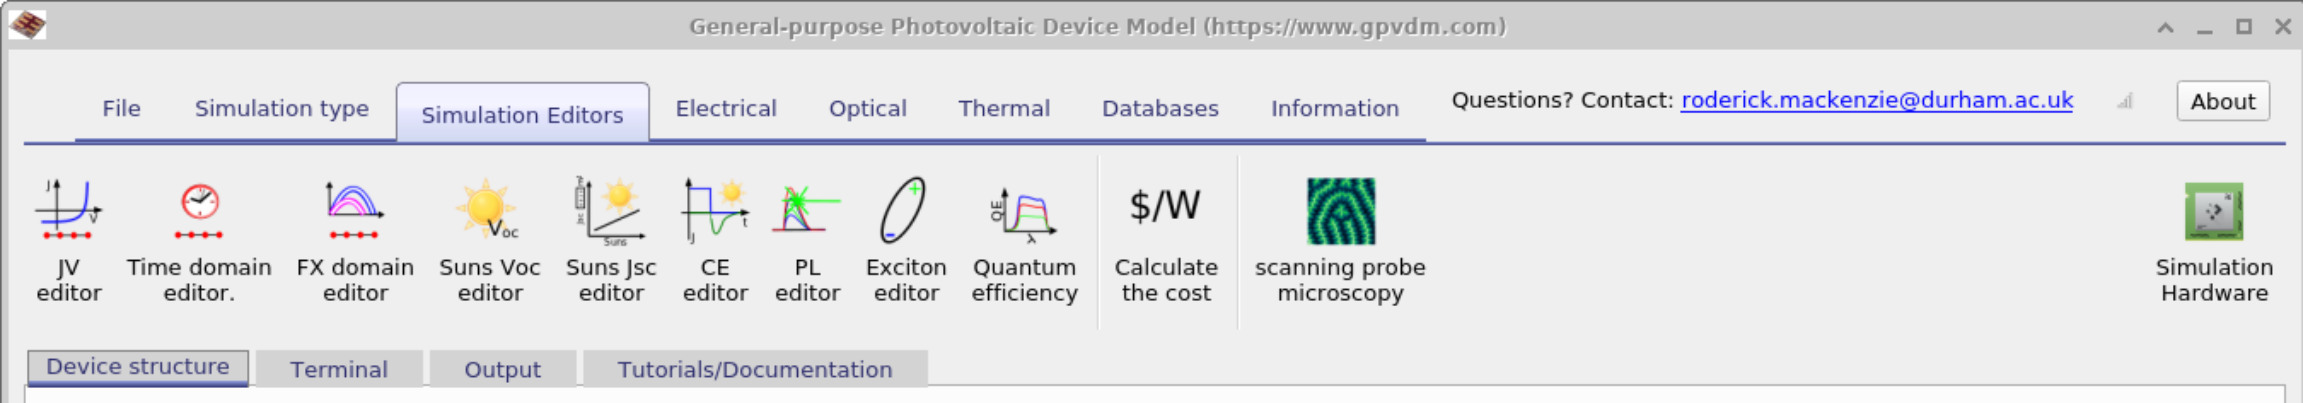
\includegraphics[width=1.0\textwidth]{./images/ribbon_sim_editors.png}
\caption{Simulation editors}
\label{fig:simeditors}
\end{figure}

Each plugin editor can generate multiple simulation modes.  For example the time domain simulation editor (see figure \ref{fig:simeditors}) is responsible for the generating both the "CELIV" and the "TPC 400mV DARK" icon in Figure \ref{fig:simmodes}. This enables the user to define new types of simulation modes at will. Below the vairous simulation editors are described.

\begin{figure}[H]
\centering
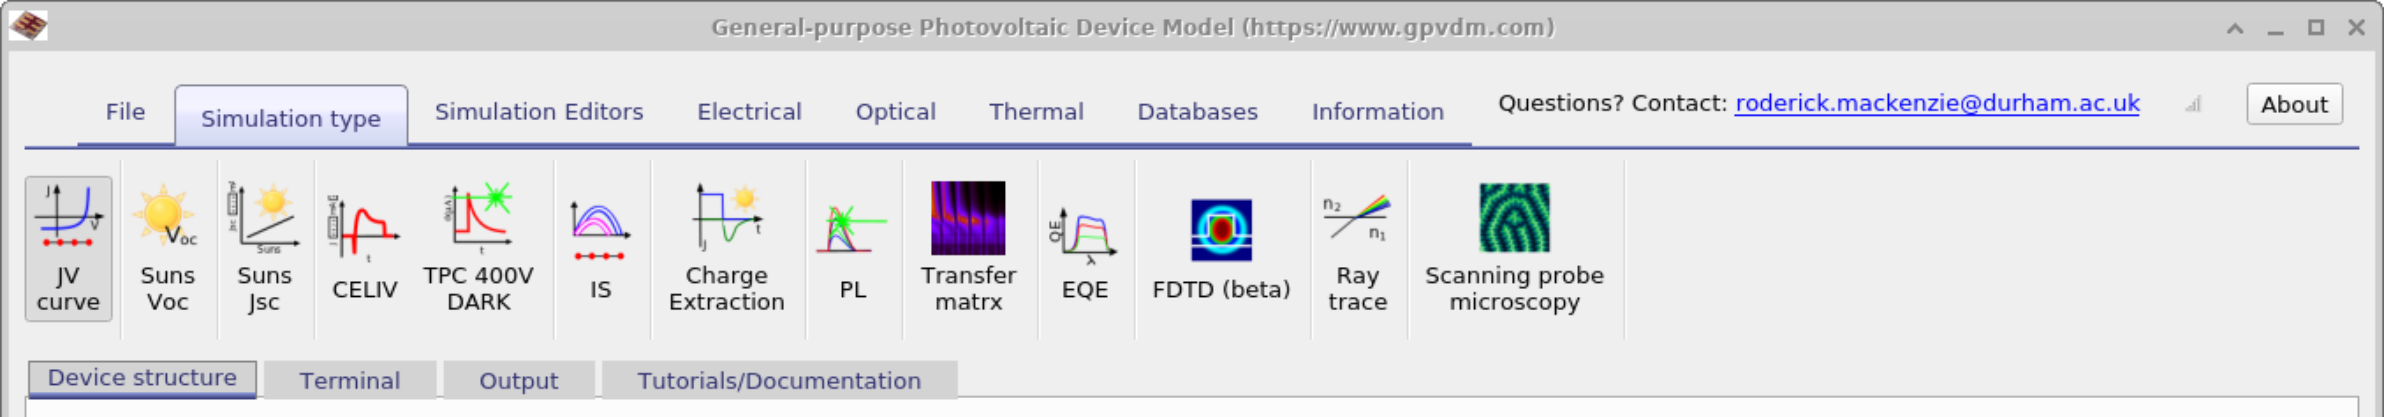
\includegraphics[width=1.0\textwidth]{./images/ribbon_sim_modes.png}
\caption{Selectig a simulation mode}
\label{fig:simmodes}
\end{figure}

\subsection{JV editor}
The JV editor icon in figure \ref{fig:simeditors} will bring up the JV editor window see figure \ref{fig:jvcurveeditor}. This window can be used to set the start and stop voltage of simulations. You can set stop currents and the by how much the voltage step grows each simulation step as well as other parameters.

\begin{figure}[H]
\centering
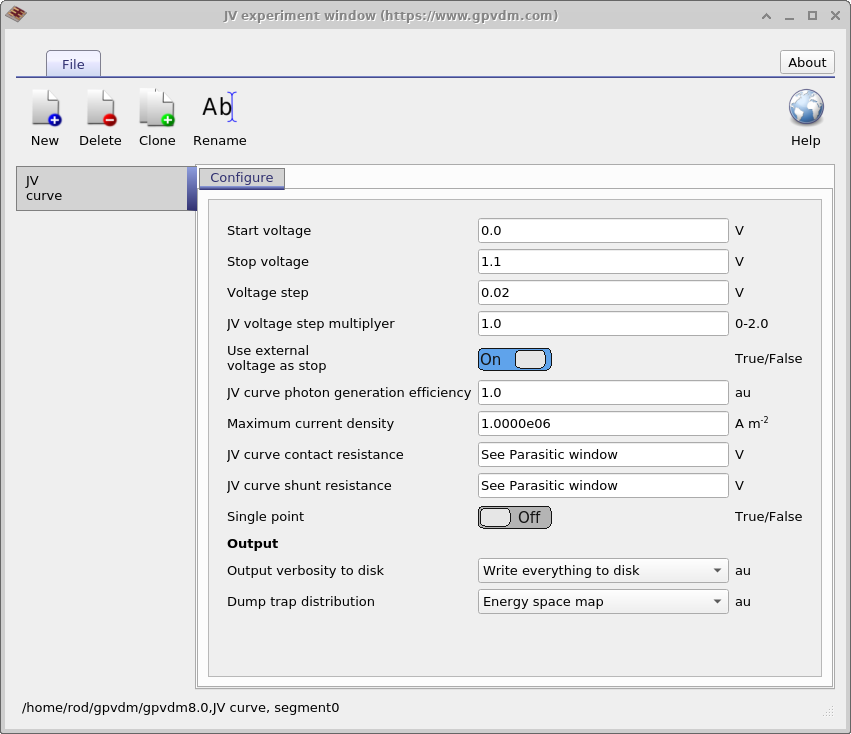
\includegraphics[width=0.7\textwidth,height=0.5\textwidth]{./images/jv_editor.png}
\caption{The JV curve editor window}
\label{fig:jvcurveeditor}
\end{figure}

\subsection{Time domain editor}
The time domain editor can be used to configure time domain simulations, this is shown in \ref{fig:timedomaineditor}.  You can see that one simulation editor can be used to edit multiple simulations.  The panel on the left shows the editor being used to edit a CELIV simulation while the panel on the right shows the editor being used to edit a TPC simulation.  The new, delete and clone buttons in the top of the window can be used to make new simulation modes. The table in the bottom of the window can be used to setup the time domain mesh, apply voltages or light.

\begin{figure}[H]
\centering
\begin{tabular}{ c c }

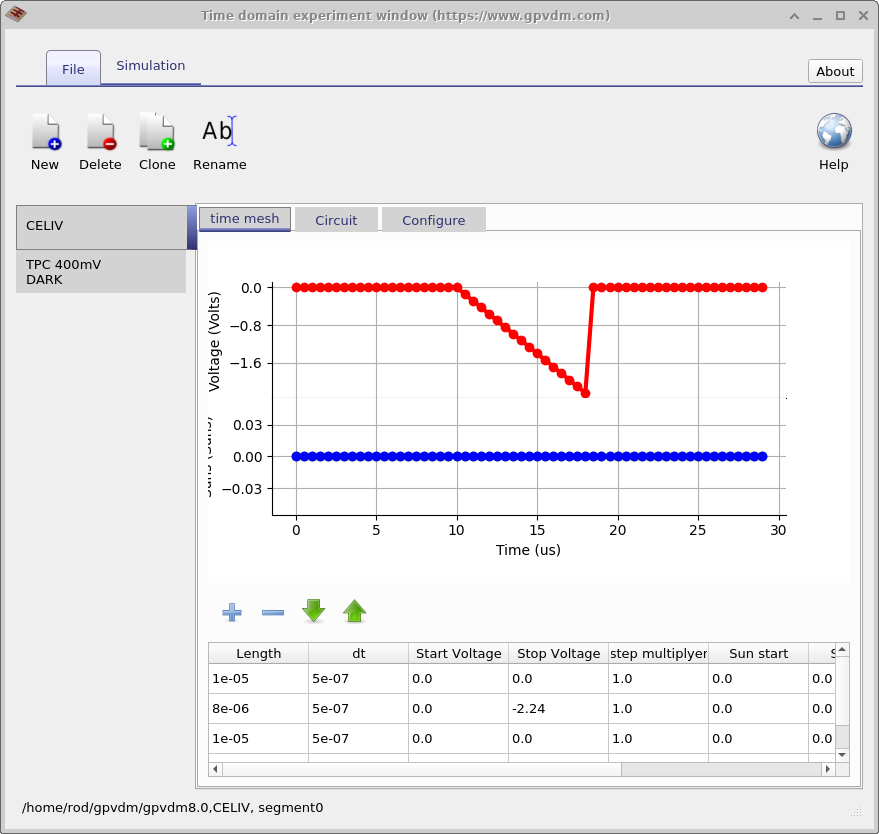
\includegraphics[width=0.5\textwidth,height=0.4\textwidth]{./images/time_domain_editor.png}

&
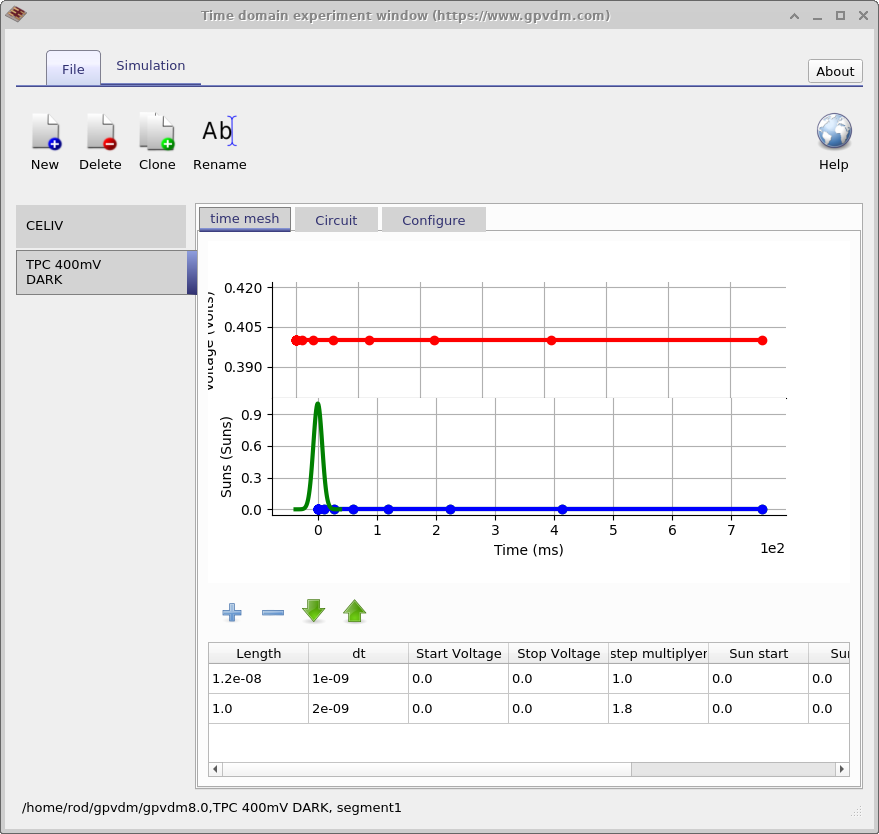
\includegraphics[width=0.5\textwidth,height=0.4\textwidth]{./images/time_domain_editor2.png}

\\

\end{tabular}
\caption{The time domain editor showing the user editing the duration of light/voltage pulses.}
\label{fig:timedomaineditor}
\end{figure}

Figure \ref{fig:timedomaineditor2} shows different tabs in of the time domain editor. The image on the left shows the circuit diagram used to model the CELIV experiment. From the left of the image the diode on the left accounts for the drift diffusion simulations it is in effect a perfect diode.  Then comes a capacitor used to model the charge on the plates of the device, then a shunt resistance and then the series resistance.  The final resistor on the right represents the external resistance of the measuring equipment.  The right hand figure shows the configuration options of the time domain window.

\begin{figure}[H]
\centering
\begin{tabular}{ c c }

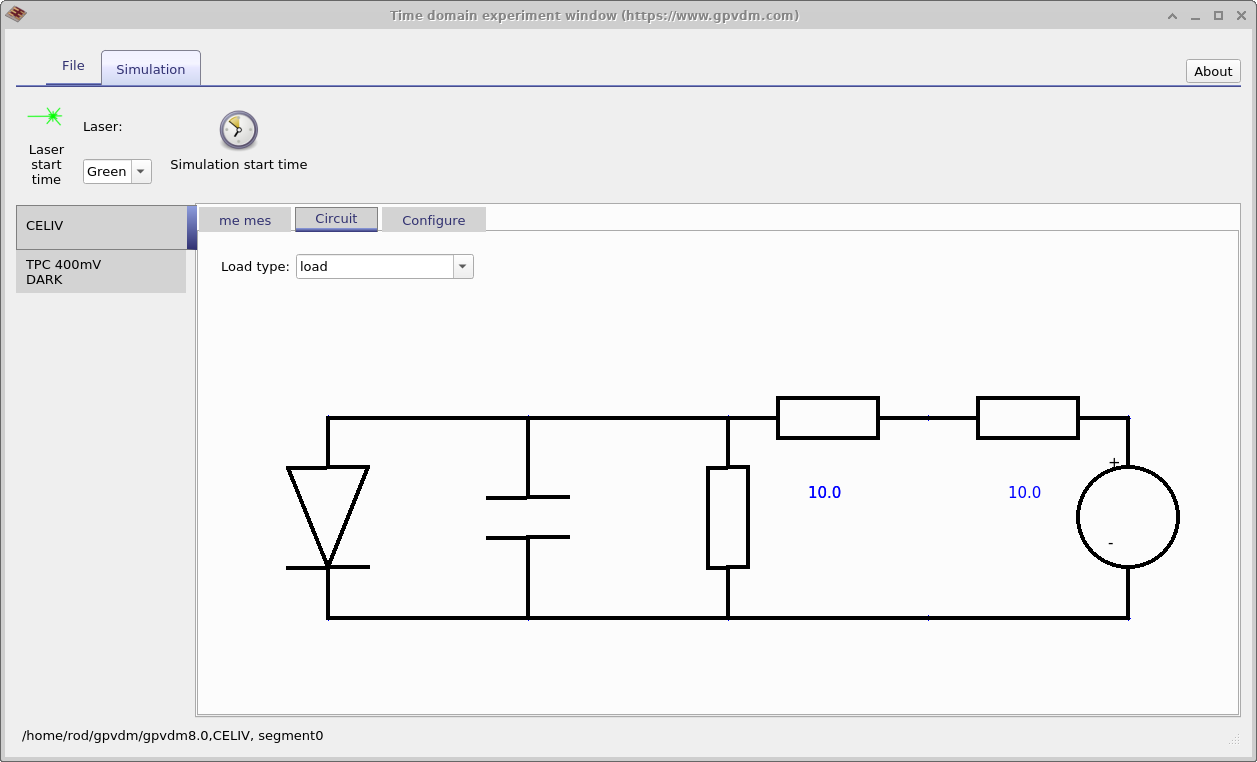
\includegraphics[width=0.5\textwidth,height=0.4\textwidth]{./images/time_domain_editor1.png}

&
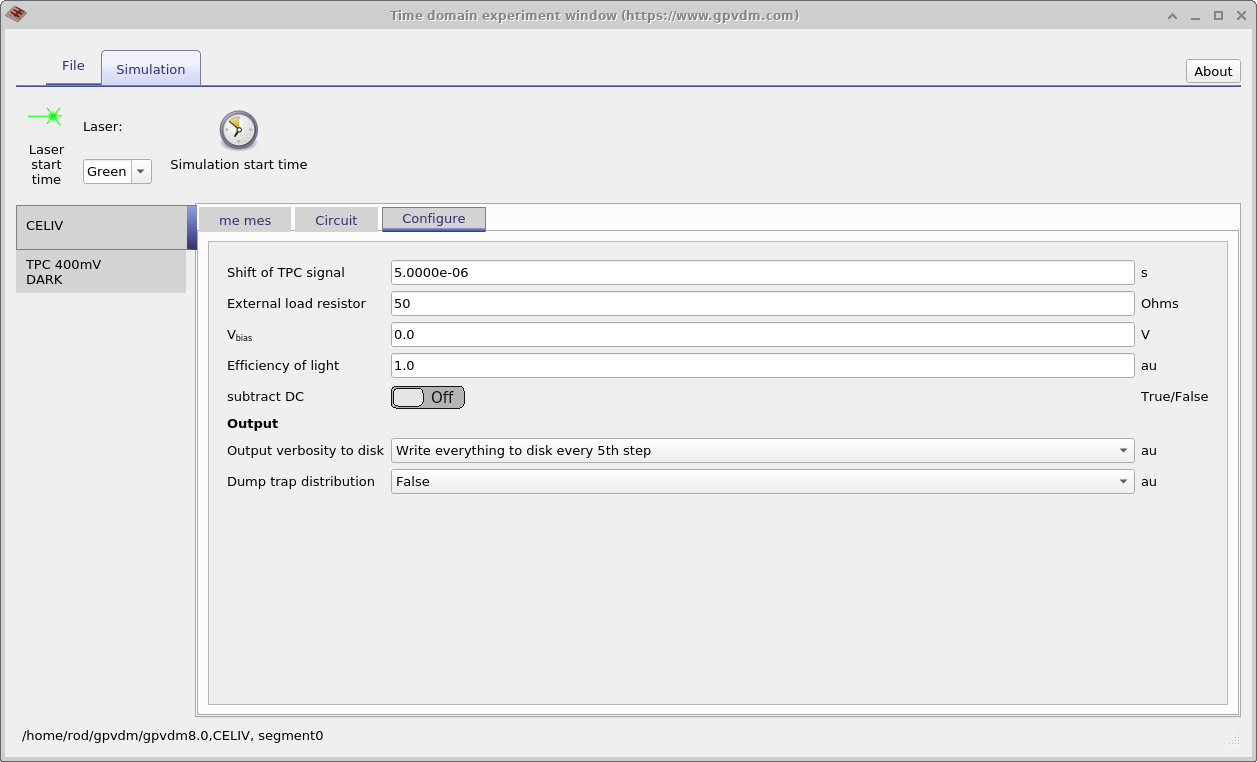
\includegraphics[width=0.5\textwidth,height=0.4\textwidth]{./images/time_domain_editor4.png}

\\

\end{tabular}
\caption{Configuring the time domain editor}
\label{fig:timedomaineditor2}
\end{figure}

\subsection{Suns-Voc editor}
The Suns-Voc plugin can be used to calculate how open circuit voltage changes as a function of light intensity.  This can be useful for understanding tail slope and disorder in devices.  A picture of the suns-voc editor window can be seen below in figure \ref{fig:sunsvoceditor}.  The window can be used to set the start and stop light intensity.

\begin{figure}[H]
\centering
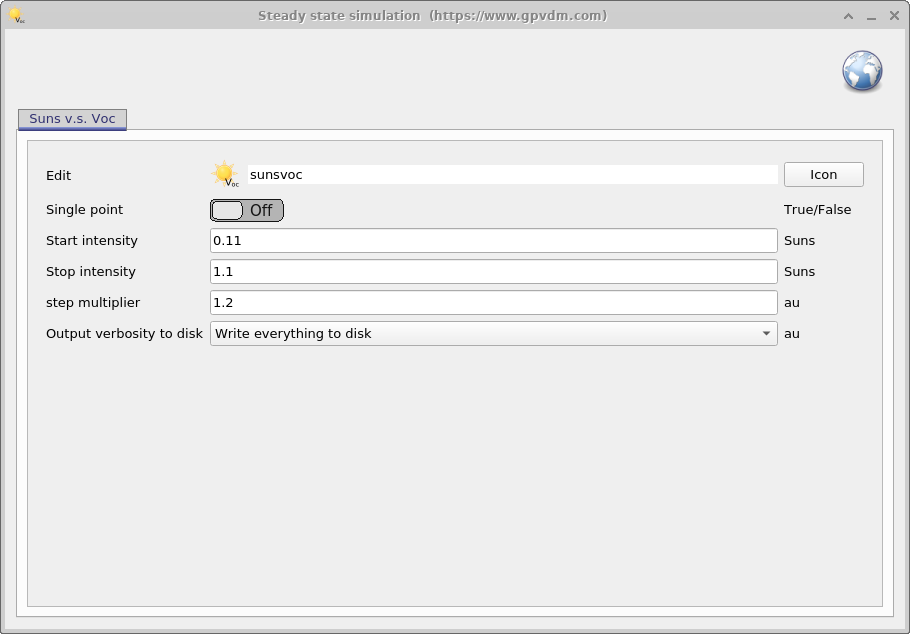
\includegraphics[width=0.7\textwidth,height=0.5\textwidth]{./images/suns_voc_editor.png}
\caption{The suns-voc editor window}
\label{fig:sunsvoceditor}
\end{figure}


\subsection{Suns-Jsc editor}
The Jsc editor can be used to configure suns-Jsc simulations. It enables you to set the start light intensity, stop light intensity and how big the steps are. This is shown in figure \ref{fig:sunsjsceditor}.

\begin{figure}[H]
\centering
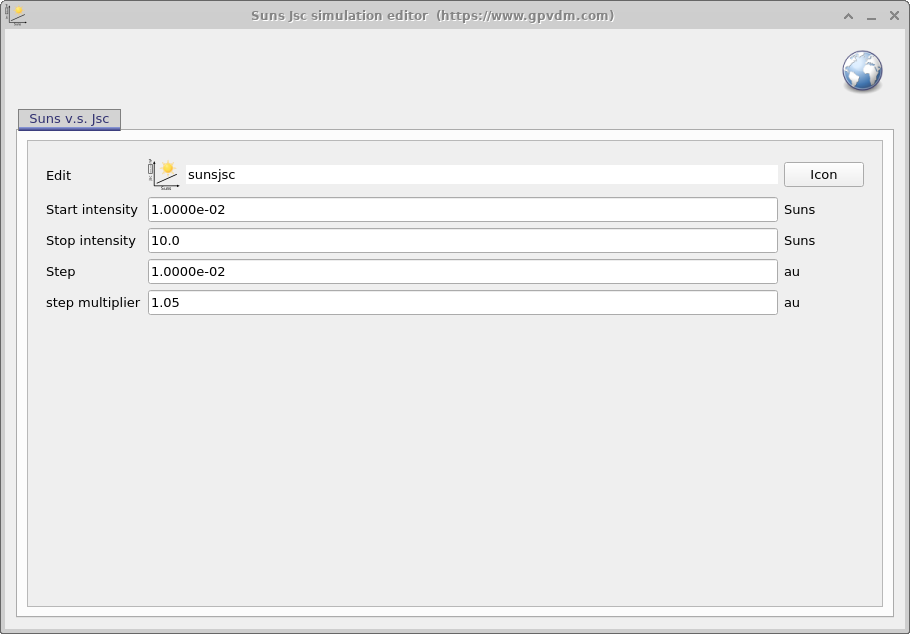
\includegraphics[width=0.7\textwidth,height=0.5\textwidth]{./images/suns_jsc_editor.png}
\caption{The JV curve editor window}
\label{fig:sunsjsceditor}
\end{figure}


\subsection{Frequency domain editor}
The frequency domain editor allows you to configure frequency domain simulations. This is shown in figure \ref{fig:fxdomaineditor}. On the right of the window you can see the frequency points which will be simulated. These are also displayed on the graph to the right of the window.  Notice that in the figure there are multiple simulations configured, IMPS, IMVS, IS and "test".  Each of these simulations will appear as an separate simulation mode in the simulation mode ribbon.

\begin{figure}[H]
\centering
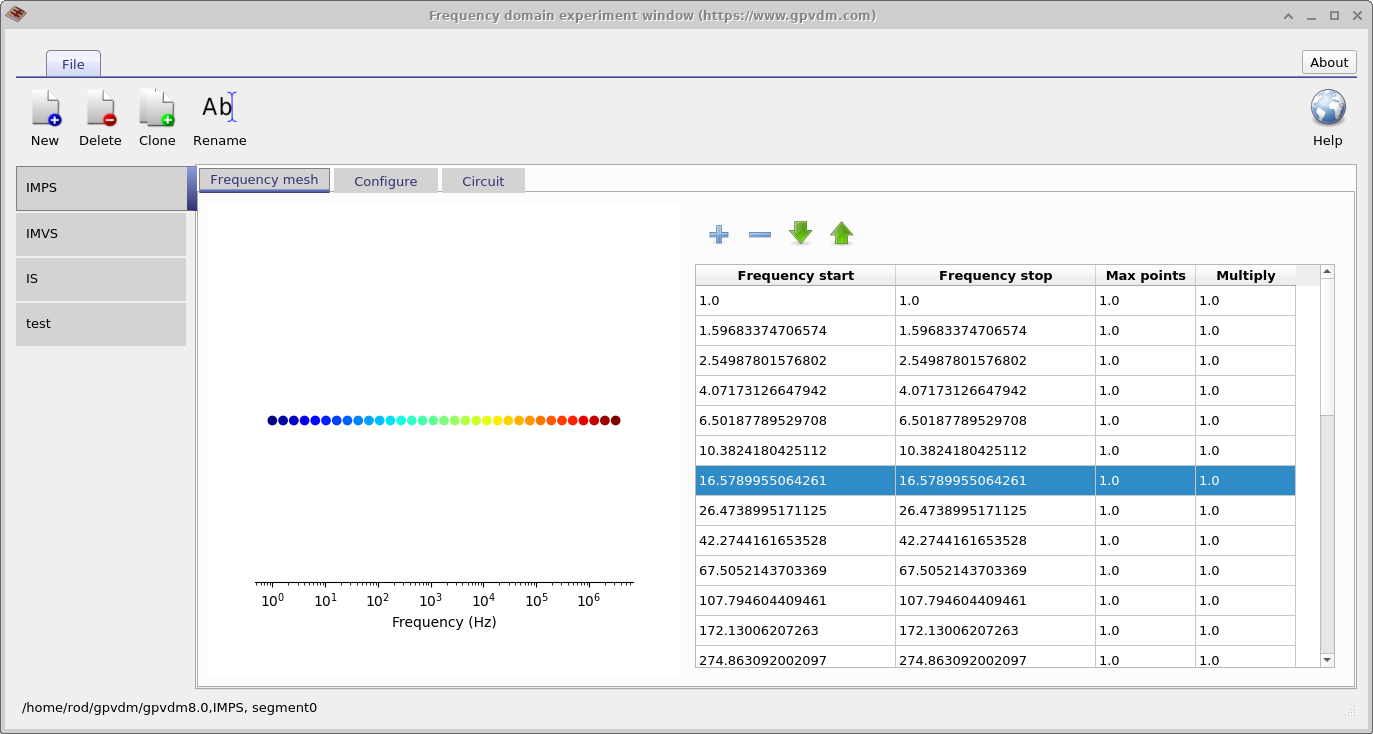
\includegraphics[width=0.7\textwidth,height=0.5\textwidth]{./images/fx_domain_editor.png}
\caption{The frequency domain editor window}
\label{fig:fxdomaineditor}
\end{figure}

\subsection{Quantum efficiency editor}
The quantum efficiency editor simulates both EQE and IQE.  The configuration window can be used to set the voltage at which EQE and IQE are performed.
\begin{figure}[H]
\centering
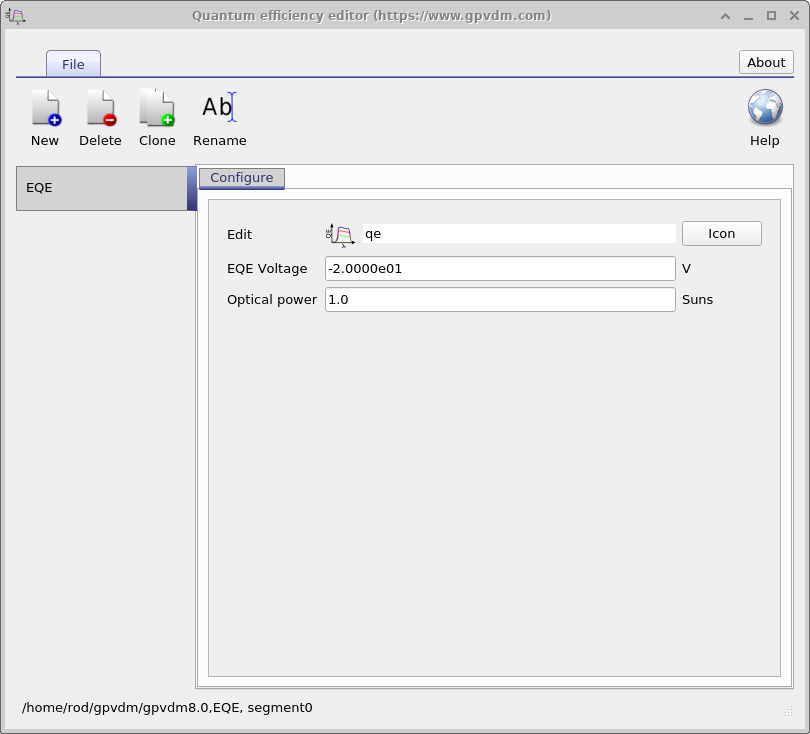
\includegraphics[width=0.7\textwidth,height=0.5\textwidth]{./images/qe_editor.png}
\caption{The quantum efficiency editor window}
\label{fig:qeeditor}
\end{figure}


